%
% reihen.tex
%
% (c) 2019 Prof Dr Andreas Müller, Hochschule Rapperswil
%
\section{Fourier-Reihen
\label{section:fourier-reihen}}
\rhead{Fourier-Reihen}
Joseph Fourier publizierte 1922 seine {\em Théorie analytique de la chaleur},
\index{Fourier, Joseph}
in der er die zeitliche Änderung der Temperaturverteilung mit Hilfe einer
partiellen Differentialgleichung beschrieb und dann eine Lösung als
Linearkombination von Sinus- und Kosinus-Funktionen konstruierte. 
Er wählte Sinus- und Kosinus-Funktionen, weil diese besonders gut in
seine Differentialgleichungen zweiter Ordnung passten.

Für unsere Untersuchung ist vor allem wichtig, dass die Sinus- und
Kosinus-Funktionen offenbar eine geeignete Funktionenmenge für die
Beschreibung eines Hilbertraums von periodischen Funktionen sind.

In diesem Abschnitt geht es daher um $2\pi$-periodische Funktionen,
also Funktionen $f\colon \mathbb R\to \mathbb R$ (oder auch
$f\colon\mathbb R\to \mathbb C$),
für die $f(t+2\pi)= f(t)$ gilt für alle $t\in\mathbb R$.  
Solche Funktionen sind natürlich nicht integrierbar, sie passen also
in dieser Form nicht in den Rahmen, den wir bisher in diesem Kapitel
entwickelt haben.
Die Periodizität bedeutet aber auch, dass die Funktionswerte für
$t\in[0,2\pi)$ die Funktion bereits vollständig beschreiben.
Umgekehrt kann man aus einer beliebigen Funktion auf dem Intervall
$[0,2\pi)$ dadurch eine Funktion auf ganz $\mathbb R$ machen, indem
man sie periodisch fortsetzt.

Die Sinus-Funktion $\sin t$ ist $2\pi$-periodisch, aber auch 
$\sin kt$ für ganzzahlige $k$.
Ebenso sind die Funktionen $\cos kt$ $2\pi$-periodisch für ganzzahlige $k$.
Da $\sin(-kt)=-\sin kt$ und $\cos(-kt)=\cos kt$ brauchen wir nur die
natürlichen $k$ zu berücksichtigen.
Dies sind die Funktionen, die Fourier verwendet hat und es sind die
Funktionen, die wir meinen, wenn wir von ``den Sinus- und Kosinus-Funktionen''
sprechen.
Um die Notation etwas zu vereinheitlichen, schreiben wir auch $s_k$ für
die Funktion $s_k(t)=\sin kt$ und $c_k$ für $c_k(t)=\cos kt$.

Der natürliche Rahmen ist daher der Hilbertraum $L^2([0,2\pi])$.
Und im Lichte des Analyse-Gedankens des ersten Kapitels stellt sich
die Frage, ob die Sinus- und Kosinus-Funktionen eine Hilbert-Basis
von $L^2([0,2\pi])$ bilden.

\subsection{Reelle Fourier-Reihen}
\label{subsection:real-fourier-series}
Wir verwenden weiterhin das Skalarprodukt
\[
\langle f,g\rangle
=
\int_0^{2\pi} f(t) \bar{g}(t)\,dt
\]
des Hilbertraums $L^2([0,2\pi])$.
Wir müssen jetzt untersuchen, ob die Sinus- und Kosinus-Funktionen
ein Erzeugendensystem bilden und ob sie orthonormiert sind.

Wir müssen daher alle Skalarprodukte von Sinus- und Kosinus-Funktionen
berechnen.
\index{Orthogonalität der trigonometrischen Funktionen}%
Dazu verwenden wir die goniometrischen Formeln, die Produkte von
trigonometrischen Funktionen durch Linearkombinationen anderer
trigonometrischer Funktionen ausdrücken:
\begin{align*}
\sin\alpha\cdot \sin\beta
&=
\frac12 \cos(\alpha-\beta) - \frac12\cos(\alpha+\beta)
&&\Rightarrow&
\sin kt \sin lt
&=
\frac12 \cos(k-l)t - \frac12\cos(k+l)t
\\
\cos\alpha \cos\beta
&=
\frac12\cos(\alpha-\beta) +\frac12\cos(\alpha+\beta)
&&\Rightarrow&
\cos kt \cos lt
&=
\frac12\cos(k-l)t + \frac12\cos(k+l)t
\\
\sin\alpha\cos\beta
&=
\frac12\sin(\alpha-\beta) + \frac12\sin(\alpha+\beta)
&&\Rightarrow&
\sin kt\cos lt
&=
\frac12\sin(k-l)t + \frac12\sin(k+l)t
\end{align*}
Damit können die Skalarprodukte der Funktionen $c_k$ und $s_k$ für natürliche
$k$ leicht berechnet werden.
Wir betrachten zunächst den Fall $k\ne l$:
\begin{align*}
\langle s_k, s_l\rangle
&=
\int_0^{2\pi} \sin kt\, \sin lt \,dt
=
\frac12\int_0^{2\pi} \cos(k-l)t\,dt
-
\frac12\int_0^{2\pi} \cos(k+l)t\,dt
\\
&=
\frac12\biggl[ \frac{\sin(k-l)t}{k-l} \biggr]_0^{2\pi}
-
\frac12\biggl[ \frac{\sin(k+l)t}{k+l} \biggr]_0^{2\pi}
=
0
\\
\langle c_k, c_l\rangle
&=
\int_0^{2\pi} \cos kt\, \cos lt \,dt
=
\frac12\int_0^{2\pi}\cos(k-l)t\,dt
+
\frac12\int_0^{2\pi}\cos(k+l)t\,dt
\\
&=
\frac12\biggl[ \frac{\sin (k-l)t}{k-l}\biggr]_0^{2\pi}
+
\frac12\biggl[ \frac{\sin (k+l)t}{k+l}\biggr]_0^{2\pi}
=
0
\\
\langle s_k, c_l\rangle
&=
\int_0^{2\pi} \sin kt\, \cos lt \,dt
=
\frac12\int_0^{2\pi} \sin(k-l)t\,dt
+
\frac12\int_0^{2\pi} \sin(k+l)t\,dt
\\
&=
\frac12\biggl[-\frac{\cos(k-l)t}{k-l}\biggr]_0^{2\pi}
+
\frac12\biggl[-\frac{\cos(k+l)t}{k+l}\biggr]_0^{2\pi}
=
0
\end{align*}
Alle diese Integrale verschwinden, weil die Stammfunktionen wieder
$2\pi$-periodische Funktionen sind.

Für $k=l>0$ erhält man dagegen
\begin{align*}
\langle s_k, s_k\rangle
&=
\int_0^{2\pi} \sin^2 kt \,dt
=
\frac12\int_0^{2\pi} 1 - \cos2kt\,dt
\\
&=
\pi
-
\frac12\biggl[ \frac{\sin2kt}{2k} \biggr]_0^{2\pi}
=
\pi
\\
\langle c_k, c_l\rangle
&=
\int_0^{2\pi} \cos^2 kt \,dt
=
\frac12\int_0^{2\pi} 1 + \cos(k+l)t\,dt
\\
&=
\pi
+
\frac12\biggl[ \frac{\sin 2kt}{2k}\biggr]_0^{2\pi}
=
\pi
\\
\langle s_k, c_k\rangle
&=
\int_0^{2\pi} \sin kt\, \cos kt \,dt
=
0
+
\frac12\int_0^{2\pi} \sin 2k t\,dt
\\
&=
\frac12\biggl[-\frac{\cos2kt}{2k}\biggr]_0^{2\pi}
=
0
\end{align*}
Die Funktionen $s_k$ und $c_l$ sind also tatsächlich orthogonal, aber
die Normierung stimmt nicht.
Dies ist leicht zu korrigieren, die Funktionen
\[
\frac1{\sqrt{\pi}} c_k(t) = \frac{1}{\sqrt{\pi}} \cos kt
\qquad\text{und}\qquad
\frac1{\sqrt{\pi}} s_k(t) = \frac{1}{\sqrt{\pi}} \sin kt
\]
sind orthonormiert.

Die konstanten Funktion $c_0(t)=1$ sollten wir noch etwas genauer untersuchen.
Es ist klar, dass $\langle c_0,s_k\rangle = 0$ und $\langle c_0,c_k\rangle=0$
für alle $k>0$, weil $c_0(t)s_k(t)=s_k(t)$ und $c_0(t)c_k(t)=c_k(t)$.
Die Norm von $c_0$ ist
\begin{align*}
\|c_0\|^2&=\langle c_0,c_0\rangle = \int_0^{2\pi}\,dt = 2\pi.
\end{align*}
Also ist auch $c_0$ nicht korrekt normiert, wir müssen stattdessen
\[
\frac1{\|c_0\|}c_0 = \frac{1}{\sqrt{2\pi}}
\]
verwenden.

Die Menge der Funktionen
\[
\mathcal{B}
=
\biggl\{
\biggl.
\frac1{\sqrt{2\pi}}, \;
\frac1{\sqrt{\pi\mathstrut}} \cos kt,\;
\frac1{\sqrt{\pi\mathstrut}} \sin kt
\;
\biggr|
\;
k>0
\biggr\}
\]
ist somit ein orthogonormiertes Funktionensystem.
Man kann zeigen, dass die Funktionen sogar ein Erzeugendensystem sind
und damit eine Hilbertbasis.
Aus den allgemeinen Prinzipien von Kapitel~\ref{chapter:geometrie}
folgt jetzt, dass sich jede Funktion in $L^2([0,2\pi])$
durch eine konvergente Reihe
aus Vielfachen der Funktionen von $\mathcal{B}$ darstellen lässt.
Die Koeffizienten sind die Skalarprodukte, also
\begin{align*}
\tilde{a}_0
&=
\frac{1}{\sqrt{2\pi}}
\int_0^{2\pi} f(t)\,dt
\\
\tilde{a}_k 
&=
\frac{1}{\sqrt{\pi\mathstrut}}
\int_0^{2\pi} f(t) \cos kt\,dt
\\
\tilde{b}_k 
&=
\frac{1}{\sqrt{\pi\mathstrut}}
\int_0^{2\pi} f(t) \sin kt\,dt,
\end{align*}
und die Reihe ist
\[
f(t)
=
\tilde{a}_0 \cdot \frac1{\sqrt{2\pi}}
+
\sum_{k=1}^\infty\biggl(
\tilde{a}_k \frac1{\sqrt{\pi\mathstrut}} \cos kt
+
\tilde{b}_k \frac1{\sqrt{\pi\mathstrut}} \sin kt
\biggr).
\]
Die Brüche in der Reihe stören etwas, daher ist es üblich, die Koeffizienten
so zu definieren, dass diese zusätzlichen Faktoren bis auf die $2$ im
Nenner von $\tilde{a}_0$ bereits in die Koeffizienten integriert sind, also
\begin{align*}
a_0
&=
\sqrt{\frac{2}{\pi}}
\tilde{a}_0
=
\frac1{\pi\mathstrut} \int_0^{2\pi} f(t)\,dt,
\\
a_k
&=
\frac{1}{\sqrt{\pi\mathstrut}} \tilde{a}_k
=
\frac1{\pi\mathstrut} \int_0^{2\pi} f(t) \cos kt\,dt
\qquad\text{und}
\\
b_k
&=
\frac{1}{\sqrt{\pi\mathstrut}} \tilde{b}_k
=
\frac1{\pi\mathstrut} \int_0^{2\pi} f(t) \sin kt\,dt.
\end{align*}
Die Reihe bekommt dann die Form
\[
f(t)
=
\frac{a_0}2
+
\sum_{k=1}^\infty \bigl( a_k \cos kt + b_k \sin kt \bigr).
\]
Dies ist die übliche Form der Fourier-Reihe.

\begin{figure}
\centering
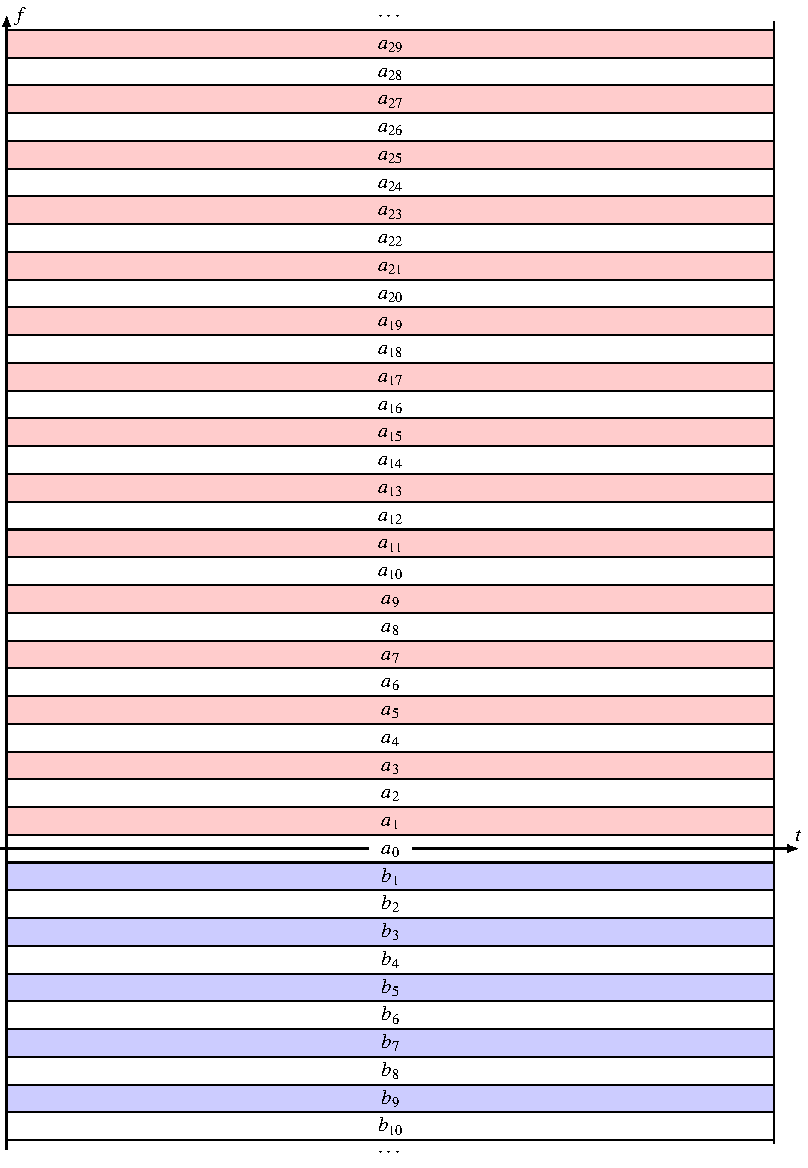
\includegraphics{chapters/2-fourier/images/ft.pdf}
\caption{Aufteilung der Frequenz-Zeit-Ebene für Fourierreihen.
\label{ft:ftplane}}
\end{figure}

Für jedes $k>0$ gibt es daher je einen Koeffizienten $a_k$ und $b_k$,
der das Verhalten des Signals bei der Frequenz $k$ wiedergibt.
Für $k=0$ gibt es genau einen Koeffizienten, nämlich $a_0$, der das
zeitunabhängige Verhalten codiert.
In der Frequenz-Zeit-Ebene lässt sich dieser Sachverhalt wie in 
Abbildung~\ref{ft:ftplane} darstellen.

\subsection{Komplexe Fourier-Reihen}
\label{subsection:complex-fourier-series}
Eine reelle Funktion in $L^2([0,2\pi])$ lässt sich mit einer Fourier-Reihe
darstellen, deren Koeffizienten alle reell sind.
Für eine komplexe Funktion werden auch die Koeffizienten komplex sein.
Die Form einer reellen Fourier-Reihe ist jetzt nicht mehr unbedingt
vorteilhaft, da die Funktionen $s_k$ und $c_k$ ziemlich unsymmetrisch
sind.
Gesucht ist daher eine orthonormiertes Erzeugendensystem aus
$2\pi$-periodischen komplexen Funktionen.
Die Eulersche Gleichung $e^{it} = \cos t + i\sin t$ deutet an, dass
dafür die Funktionen
\[
e_k(t) = e^{ikt}
\]
geeignet sein könnten.
Es ist bereits jetzt klar, dass diese Funktionen ein Erzeugendensystem
bilden, denn es lassen sich daraus mit
\[
\cos kt = \frac{e^{ikt}+e^{-ikt}}2
\qquad\text{und}\qquad
\sin kt = \frac{e^{ikt}-e^{-ikt}}{2i}
\]
alle Funktionen des Erzeugendensystems
der reellen Fourier-Reihen linear kombinieren.
Es bleibt also nur noch sicherzustellen, dass sie auch orthonormiert
sind.
Dazu werden wieder die Skalarprodukte berechnet.
Zunächst gilt für $k\ne l$
\begin{align*}
\langle e_k,e_l\rangle
&=
\int_0^{2\pi} e_k(t) \bar{e}_l(t) \,dt
=
\int_0^{2\pi} e^{ikt}e^{-ilt}\,dt
=
\int_0^{2\pi} e^{i(k-l)t}\,dt
=
\biggl[ \frac{e^{i(k-l)t}}{i(k-l)} \biggr]_0^{2\pi} 
=
0,
\end{align*}
die Funktionen sind also orthogonal.
Sie sind aber nicht normiret, denn für $k=l$ ist 
\[
\|e_k\|^2
=
\int_0^{2\pi} e^{ikt}e^{-ikt}\,dt
=
\int_0^{2\pi} \,dt = 2\pi.
\]
Um die Funktionen zu normieren, muss man also durch $\sqrt{2\pi}$ teilen.

Es folgt also, dass die Funktionen
\[
\mathcal{C}
=
\biggl\{
\frac1{\sqrt{2\pi}} e_k(t)
=
\frac1{\sqrt{2\pi}} e^{ikt}\;\bigg|\; k\in\mathbb Z
\biggr\}
\]
eine Hilbertbasis von $L^2([0,2\pi])$ bilden.
Die Koeffizienten sind 
\[
\tilde{c}_k 
=
\langle f, e_k\rangle
=
\frac1{\sqrt{2\pi}}
\int_0^{2\pi} f(t) e^{-ikt}\,dt
\]
und die zugehörige Reihe ist
\[
f(t)
=
\sum_{k=1} \tilde{c}_k \frac{1}{\sqrt{2\pi}} e^{ikt}.
\]
Wie im Falle der reellen Fourier-Reihe ist es auch bei der komplexen
Fourier-Reihe üblich, die Koffizienten so zusammenzufassen, dass in der
Fourier-Reihe keine Faktoren der Form $1/\sqrt{2\pi}$ nötig sind, also
\[
c_k
=
\frac1{\sqrt{2\pi}} \tilde{c}_k
=
\frac1{2\pi} \int_0^{2\pi} f(t) e^{-ikt}\,dt.
\]
Damit wird die Fourier-Reihe dann
\[
f(t) = \sum_{k\in\mathbb Z} c_k e^{ikt}.
\]

\subsection{Plancherel-Formel}
Da die Funktionen $\mathcal{B}$ eine Hilbertbasis bilden, können wir sofort
schliessen, dass die $L^2$-Norm $\|f\|$ einer Funktion $f\in L^2([0,2\pi])$
auch mit den Fourier-Koeffizienten berechnet werden kann.
Für eine Hilbertbasis ist die $L^2$-Norm $\|f\|^2$ ist die Quadratsumme
der Koeffizienten $|\langle f,b_i\rangle|^2$.
Für die Fourier-Reihe folgt daher
\[
\| f \|^2
=
|\tilde{a}_0|^2
+
\sum_{k=1}^\infty
(
|\tilde{a}_k|^2
+
|\tilde{b}_k|^2
)
=
\frac{\pi}{2}
|a_0|^2
+
\pi
\sum_{k=1}^\infty
(
|a_k|^2
+
|b_k|^2
)
\]
Dasselbe gilt natürlich auch für die komplexe Fourierreihe.
Dort gilt
\[
\| f\|^2
=
\sum_{k\in\mathbb Z} |\tilde{c}_k|^2
=
2\pi \sum_{k\in\mathbb Z} |c_k|^2.
\]

\subsection{Lokalisierung
\label{fourier:reihen:lokalisierung}}
\index{Lokalisierung}%
Wie änderen sich die komplexen Fourier-Koeffizienten $c_k$, wenn die
Funktion an einer Stelle modifiziert wird?
Zunächst ist ein einzelner Punkt eine Nullmenge und damit äussert sich
eine solche Änderung im Skalarprodukt nicht.
Wir können aber eine Folge $\delta_n$ von $L^2$ Funktionen mit beliebig
kleinem Träger und $L^1$-Norm $1$ definieren:
\begin{equation}
\delta_n(t) = \begin{cases}
2n&\qquad-\frac1n \le t\le \frac1n\\
0&\qquad\text{sonst.}
\end{cases}
\label{fourier:deltadef}
\end{equation}
Die Funktion ist so konstruiert, dass das Integral immer $1$ ist, also
$\|\delta-n\|_1=1$ für alle $n$.

Die Fourier-Koeffizienten der Funktionen $\delta_n$ sind
\begin{equation}
\langle \delta_n,e_k \rangle
=
\frac{1}{\sqrt{2\pi}}\int_{-\pi}^\pi \delta_n(t) e^{-ik t}\,dt
=
\frac{1}{\sqrt{2\pi}}\int_{-\frac1n}^{\frac1n} e^{-ikt}\,dt
\to
\frac{1}{\sqrt{2\pi}}
\qquad\text{für $n\to\infty$}.
\label{fourier:delta0}
\end{equation}
Eine Änderung eines Signals um die Funktion $\delta_n$ ändert daher im
Grenzfall alle Fourier-Koeffizienten um $1/\sqrt{2\pi}$.

Verschieben wir die Funktion um $b$, betrachten wir also
$T_b\delta_n$, dann folgt analog
\begin{equation}
\langle T_b\delta_n,e_k\rangle
\to
\frac{1}{\sqrt{2\pi}}e^{-ikb}
\quad
\text{für $n\to\infty$}.
\label{fourier:deltab}
\end{equation}
Eine Änderung des Signals in unmittelbarer Nähe des Punktes $b$ ändert also
ebenfalls alle Fourier-Koeffizienten um eine Zahl mit Betrag
$1/\sqrt{2\pi}$, aber die Änderungen unterscheiden sich gegenüber
\eqref{fourier:delta0} um den Phasenfaktor.
Die Information über die lokaler Änderung ist also verteilt über alle
Koeffizienten und ist codiert im Phasenfaktor $e^{-ikb}$.
Man sagt auch, eine lokale Änderung ist im Frequenzbereich vollständig
delokalisiert.
\index{delokalisiert}%

Die Folge $\delta_n$ hat in $L^2$ keinen Grenzwert, kann also nicht als
Funktion betrachtet werden.
Trotzdem spricht man oft von einer {\em Delta-Funktion}.
\index{Delta-Funktion}%
\index{Dirac-$\delta$}%
Die Theorie der Distributionen gibt dem Grenzwert der Folge $\delta_n$ 
einen Sinn, muss zu diesem Zweck aber den Raum der in Frage kommenden
Funktionen von $L^2$ auf einen kleineren Raum reduzieren.
Wir benötigen diese Theorie wie auch die $\delta$-``Funktion'' im
Folgenden nicht und verzichten daher auf eine tiefergehende Darstellung.

